\documentclass[border=4pt]{standalone}
\usepackage{tikz}
\usepackage{pgfplots}
\pgfplotsset{compat=1.18}
\usetikzlibrary{arrows.meta}
\begin{document}
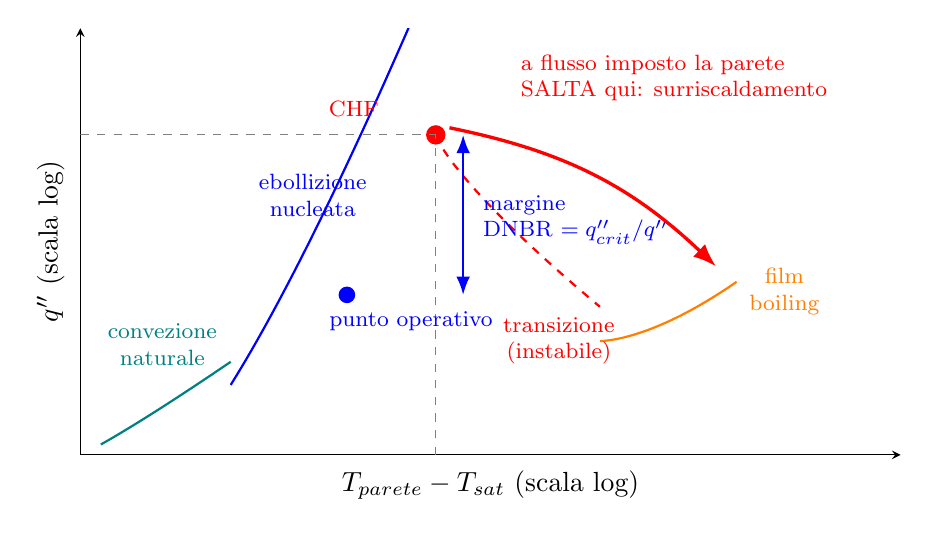
\begin{tikzpicture}
\begin{axis}[
  width=12cm, height=7cm,
  xlabel={$T_{parete}-T_{sat}$ (scala log)},
  ylabel={$q''$ (scala log)},
  xtick=\empty, ytick=\empty,
  axis lines=left,
  xmin=0, xmax=12, ymin=0, ymax=12,
]
% convection natural
\addplot[thick,teal,domain=0.3:2.2,samples=30]{1.1*x^1.1};
% nucleate boiling steep
\addplot[thick,blue,domain=2.2:5.2,samples=40]{2.6*(x-1.4)^1.25};
% transition (dashed, unstable)
\addplot[thick,red,dashed,domain=5.2:7.6,samples=30]{9.0-2.4*(x-5.2)^0.8};
% film boiling
\addplot[thick,orange,domain=7.6:9.6,samples=30]{3.2+0.55*(x-7.6)^1.6};
% CHF point
\fill[red] (axis cs:5.2,9.0) circle (3.5pt);
\node[font=\footnotesize,red,anchor=south] at (axis cs:4.0,9.25) {CHF};
\draw[dashed,gray] (axis cs:0,9.0) -- (axis cs:5.2,9.0);
\draw[dashed,gray] (axis cs:5.2,0) -- (axis cs:5.2,9.0);
% operating point
\fill[blue] (axis cs:3.9,4.5) circle (3pt);
\node[font=\footnotesize,blue,anchor=north west] at (axis cs:3.5,4.3) {punto operativo};
\draw[{Latex}-{Latex},thick,blue] (axis cs:5.6,4.5) -- (axis cs:5.6,9.0);
\node[font=\footnotesize,blue,anchor=west,align=left] at (axis cs:5.75,6.6) {margine\\ DNBR $=q''_{crit}/q''$};
% regime labels
\node[font=\footnotesize,teal,align=center] at (axis cs:1.2,3.1) {convezione\\ naturale};
\node[font=\footnotesize,blue,align=center] at (axis cs:3.4,7.3) {ebollizione\\ nucleata};
\node[font=\footnotesize,red,align=center] at (axis cs:7.0,3.2) {transizione\\ (instabile)};
\node[font=\footnotesize,orange,align=center] at (axis cs:10.3,4.6) {film\\ boiling};
% the jump
\draw[-{Latex},very thick,red] (axis cs:5.4,9.2) to[bend left=16] (axis cs:9.3,5.3);
\node[font=\footnotesize,red,anchor=west,align=left] at (axis cs:6.3,10.6) {a flusso imposto la parete\\ SALTA qui: surriscaldamento};
\end{axis}
\end{tikzpicture}
\end{document}
